\documentclass[a4paper, 11pt]{article}
\usepackage[margin=1in]{geometry}
\usepackage{amsmath}
\usepackage{graphicx}
\usepackage{tikz}
\usepackage[hidelinks]{hyperref}
\usepackage{color}
\usepackage{xcolor}
\usepackage{listings}
\usepackage{float}

\lstset{basicstyle=\small}

\usepackage{caption}
\DeclareCaptionFont{white}{\color{white}}
\DeclareCaptionFormat{listing}{\colorbox{gray}{\parbox{\textwidth}{#1#2#3}}}
\captionsetup[lstlisting]{format=listing,labelfont=white,textfont=white}

\begin{document}
%Header-Make sure you update this information!!!!
\noindent
\large\textbf{Obligatory Assignment 2 Report} \hfill \textbf{Tomasz Gliniecki} \\


\section*{Problem 1}
System works if at least 11 components work.

\emph{Simulation}:\\
\centerline{$ \sum_{15}^{i=1} I (U_i \leq p_i) \geq 11 $}

a)
simulation results: P(A) = $ 0.987 $

b)
simulation results: P(A) = $0.841$ with standard error = $0.00366$


\section*{Problem 2}

%\begin{figure}[H]
%  \centering
%  \includegraphics[scale=0.7,page=3]{Rplots.pdf}
%  \caption{Simulation of 5 lives}
%  \label{k5}
%\end{figure}

\section*{Problem 4}

a) $T_1$  and $T_2$ are exponentially distributed because we are drawing from uniform distribution and correcting it with $-ln(U_n)$ to make it exponential.

  
\begin{thebibliography}{9}
  
\bibitem{montyhall} 
  Monty Hall problem, [cited 27.September 2016]. Available at \url{https://en.wikipedia.org/wiki/Monty_Hall_problem}

\end{thebibliography}

\end{document}
